% ****** Start of file .tex ******
%
%   This file is based on apssamp.tex, part of the APS files in the REVTeX 4.1 distribution.
%   Version 4.1r of REVTeX, August 2010
%
%   Copyright (c) 2009, 2010 The American Physical Society.
%   Samuel Balula, Pedro Ribeiro, Luís Macedo, Eduardo Neto 2013
%   See the REVTeX 4 README file for restrictions and more information.
%
% TeX'ing this file requires that you have AMS-LaTeX 2.0 installed
% as well as the rest of the prerequisites for REVTeX 4.1
%
% See the REVTeX 4 README file
% It also requires running BibTeX. The commands are as follows:
%
%  1)  latex filename.tex
%  2)  bibtex filename
%  3)  latex filename.tex
%  4)  latex filename.tex

\documentclass[%
  reprint,
  %superscriptaddress,
  %groupedaddress,
  %unsortedaddress,
  %runinaddress,
  %frontmatterverbose, 
  %preprint,
  %showpacs,preprintnumbers,
  nofootinbib,
  %nobibnotes,
  %bibnotes,
  amsmath,amssymb,
  aps,
  %pra,
  %prb,
  %rmp,
  %prstab,
  %prstper,
  %floatfix,
  10pt,
  a4paper
]{revtex4-1}

\if11
% Usual (decimal) numbering
\renewcommand{\thesection}{\arabic{section}}
\renewcommand{\thesubsection}{\thesection.\arabic{subsection}}
\renewcommand{\thesubsubsection}{\thesubsection.\arabic{subsubsection}}

% Fix references
\makeatletter
\renewcommand{\p@subsection}{}
\renewcommand{\p@subsubsection}{}
\makeatother

\fi

\usepackage{listings}
\usepackage{color}
\usepackage{facil}                      % Pacote pessoal
\usepackage{verbatim}                   % Apresentação de código
\usepackage{graphicx}                   % Include figure files
\usepackage{dcolumn}                    % Align table columns on decimal point
\usepackage{bm}                         % bold math
\usepackage[latin1,utf8]{inputenc}      % Tipos de caracteres
\usepackage[portuges]{babel}            % Português
\usepackage{indentfirst}                % Identação da primeira linha
\usepackage{hyperref}                   % add hypertext capabilities
\usepackage{float}                      %Fixar imagens
 \usepackage{subcaption}
%\usepackage[mathlines]{lineno}          % Enable numbering of text and display math
%\linenumbers\relax                      % Commence numbering lines
%\usepackage[compact]{titlesec}

\usepackage[%showframe,%Uncomment any one of the following lines to test 
%%scale=0.7, marginratio={1:1, 2:3}, ignoreall, % default settings
%%text={7in,10in},centering,
margin=0.5in,        %diminuir margens
%total={6.5in,8.75in}, top=1.2in, left=0.9in, 
includefoot
%height=10in,a5paper,hmargin={3cm,0.8in},
]{geometry}

\begin{document}
%\preprint{APS/123-QED}
%\captionsetup[table]{font=small,skip=0pt}
%\captionsetup[figure]{font=small,skip=0pt}
%\titlespacing{\section}{0pt}{*0}{*0}            %Poupar espaço
%\titlespacing{\subsection}{0pt}{*0}{*0}
%\titlespacing{\subsubsection}{0pt}{*0}{*0}

\lstset{language=Matlab,%
    %basicstyle=\color{red},
	belowcaptionskip=1\baselineskip,
	frame=L,
    breaklines=true,%
    morekeywords={matlab2tikz},
    keywordstyle=\color{blue},%
    morekeywords=[2]{1}, keywordstyle=[2]{\color{black}},
    identifierstyle=\color{black},%
    stringstyle=\color{mylilas},
    commentstyle=\color{mygreen},%
    showstringspaces=false,%without this there will be a symbol in the places where there is a space
    numbers=left,%
    numberstyle={\tiny \color{black}},% size of the numbers
    numbersep=9pt, % this defines how far the numbers are from the text
    emph=[1]{for,end,break},emphstyle=[1]\color{red}, %some words to emphasise
    %emph=[2]{word1,word2}, emphstyle=[2]{style},    
}
% % % % % % % % % % % % % % % % % % % % % % % % % % % % % % % % % % % % % % % % 
%%%%%%%%%%%%%%%%%%%%%%%%%%%%%%%%%% Início %%%%%%%%%%%%%%%%%%%%%%%%%%%%%%%%%%%%%%
% % % % % % % % % % % % % % % % % % % % % % % % % % % % % % % % % % % % % % % %
 

\title{Controlo por retroacção do estado de um braço robot flexível}
\thanks{Relatório do trabalho de laboratório}
\author{Alexandre Aparício}
\email{73252, alexandre.aparicio@tecnico.ulisboa.pt}

\author{Pedro Ribeiro}%
\email{73221, pedro.q.ribeiro@tecnico.ulisboa.pt}
\author{Samuel Balula}%
\email{72735, samuel.balula@tecnico.ulisboa.pt}

\affiliation{
  Instituto Superior Técnico\\
  Mestrado em Engenharia Física Tecnológica\\
  Controlo em Espaço de Estados
}

\collaboration{Grupo 4A de 4ª feira}

\date{\today}

%%%%%%%%%%%%%%%%%%%%%%%%%%%%%%%%%% Abstract %%%%%%%%%%%%%%%%%%%%%%%%%%%%%%%%%%%%
\begin{abstract}
Neste trabalho de laboratório procede-se ao dimensionamento de um controlador por realimentação de variáveis de estado de uma barra flexível actuada por um motor dc, aproximada por um sistema linear, que inclui um observador assimptótico e seguimento de referência.
O modelo é testado em {\it simulink}, recorrendo tanto a simulações como utilizando o sistema real.
Apresentam-se neste documento os dados experimentais e as respostas às questões laboratoriais.
\end{abstract}
\maketitle


%%%%%%%%%%%%%%%%%%%%%%%%%%%%%%%%%% Introdução %%%%%%%%%%%%%%%%%%%%%%%%%%%%%%%%%%
\section{Controlabilidade}

De acordo com as informações dadas no enunciado, tomando como vector de estado $x$ dado por \eqref{x} as matrizes do modelo de estado linearizado na forma \eqref{lin} são dadas por \eqref{A}, \eqref{B} e \eqref{C}.

\eq[x]{x = \begin{bmatrix}
		x_1 &x_2 &x_3 &x_4 
\end{bmatrix} = \begin{bmatrix}
\theta & \alpha & \dot\theta& \dot\alpha
\end{bmatrix}}

\eq[lin]{\begin{cases}
	\dot x = A x + b u \\
	y = C x
\end{cases}}



\eq[A]{A = \begin{bmatrix}
		0	&0		&1		&0	\\
		0	&0		&0		&1	\\
		0	&566	&-37	&0	\\
		0	&-922	&37		&0	
\end{bmatrix}
}

\eq[B]{b= \begin{bmatrix}
		0 \\
		0\\
		65\\
		-65
\end{bmatrix}}

\eq[C]{c = \begin{bmatrix}
		1 &1	&0	&0
	\end{bmatrix}
}

Pode assim escrever-se a matrix de controlabilidade como \eqref{contr}, calculada em {\it Matlab} como se descreve em \rlis{list1}.

\eq[contr]{\begin{array}{rcl}
		\mathcal{C} &= &
		\begin{bmatrix}
			b &A b & A^2 b & A^3 b
		\end{bmatrix}\\
		&= &
		\begin{bmatrix}
			0         &65       &-2405       &52195 \\
			0         &-65        &2405      &-29055\\
			65       &-2405       &52195     &-569985\\
			-65        &2405      &-29055     &-286195
		\end{bmatrix}
	\end{array}
}

Determinou-se que o sistema é controlável (a dimensão da matriz de controlabilidade é igual ao número de variáveis de estado).

\begin{lstlisting}[label=list1, caption={Código Matlab para o cálculo da matrix de controlabilidade $\mathcal{C}$ e de observabilidade $\mathcal{O}$. As variáveis {\it cntr} e {\it obsr} adquirem valores booleanos, que indicam se o sistema é controlável e/ou observável, respectivamente. As funções {\it controlab} e {\it observab} apresentam-se em anexo em ficheiros com o mesmo nome.}]
[C,cntr]=controlab(A,b);
[O,obsr]=observab(A,c);
\end{lstlisting}


\section{Observabilidade}
A matrix de observabilidade é dada por \eqref{obsr}, calculada em {\it Matlab} como se descreve em \rlis{list1}.


\eq[obsr]{\begin{array}{rcl}
		\mathcal{O} &= &
		\begin{bmatrix}
			c \\
			c A\\
			c A^2\\
			c A^3
		\end{bmatrix}\\
		&= &
		\begin{bmatrix}
			1     &1    &0     &0\\
			0     &0     &1     &1\\
			0  &-356     &0     &0\\
			0     &0     &0  &-356
		\end{bmatrix}
	\end{array}
}
Determinou-se que o sistema é observável (a dimensão da matriz de observabilidade é igual ao número de variáveis de estado).

\section{Diagrama de Bode}
\fig{../img/BodeMalhaAberta.png}{Diagrama de Bode do sistema em cadeira aberta}

Através do diagrama de Bode da \rfig{../img/BodeMalhaAberta.png} é possível concluir que o sistema possui 4 pólos, tal como esperado. O motor DC introduz dois pólos reais\cite{dcmotor} e a barra dois pólos complexos conjugados, característicos de um movimento oscilatório amortecido.

Calcularam-se os valores próprios da matriz A, que correspondem aos pólos do sistema em cadeia aberta, que se apresentam na tabela \ref{tab1} e estão representados na \rfig{../img/OpenZeroPole.png}.

Como se pode observar, um dos pólos reais está na origem e o restante tem módulo bastante próximo do dos dois pólos complexos conjugados. O efeito destes é assim essencialmente conjunto.
\par Verifica-se no digrama de Bode que, para cerca de 4Hz dá-se uma variação de fase de -270º devida aos três pólos, que em conjunto com os -90º devidos ao pólo na origem, prefaz a diferença de fase de -360º para grandes valores de frequência. Do mesmo modo, para a amplitude observa-se um declive inicial de -20dB devido ao pólo na origem e um aumento deste em -60dB em cerca de 4Hz, prefazendo um declive de -80dB para grandes valores de frequência.

Tem-se assim que a resposta do sistema se dá para baixas frequências, apresentando atenuações superiores a 60dB para frequências superiores a 10Hz.

\tabela[tab1]{Pólos do sistema em cadeia aberta (valores própios da matriz A)}{ccc}
{
	
$z$	&$\abs{z}$	&$\abs{z}$/(2$\pi$)	\\ 	
rad $s^{-1}$	&rad $s^{-1}$	& Hz \\ \hline
$   0.0000 + 0.0000i$	&$0$	&$0$	\\
$  -7.4016 +23.2085i$	&$24.3601$	&$3.877$	\\
$  -7.4016 -23.2085i$	&$24.3601$	&$3.877$	\\
$ -22.1969 + 0.0000i$	&$22.1969$	&$3.5327$


}

\fig{../img/OpenZeroPole.png}{Pólos do sistema em cadeia aberta, respresentados no plano complexo.}

\par Ainda relativamente ao sistema em malha aberta e construiu-se o gráfico da \rfig{../img/OpenRootLocus.png}, recorrendo à função \verb+rlocus()+ do Matlab.

\fig{../img/OpenRootLocus.png}{\textit{Root Locus} do sistema em malha aberta.}

\par Na perspectiva do \textit{root locus} podem observar-se as trajectórias dos quatro pólos no plano complexo quando o ganho é variado. Desta forma, o ganho do controlador do sistema poderia ter sido desenhado procedendo à escolha dos pólos que respeitariam uma certa condição a impor. Por outras palavras, conforme o comportamento a impor ao sistema ou a resposta desejada do mesmo, o ganho (controlador proporcional) seria escolhido conforme a nova localização para os pólos.
\par O gráfico evidencia propriedades características do \textit{root locus}, como esperado, nomeadamente a simetria relativa ao eixo real e o ângulo de abertura dos pólos. Pode ainda observar-se que quando o ganho chega a um certo valor, os pólos oscilatórios cruzam o eixo imaginário, ficando com parte real positiva, logo instáveis. Relativamente aos pólos reais, com módulo negativo, estes, a partir de um certo valor de ganho tornam-se complexos conjugados, introduzindo mais oscilações ao sistema. Ainda antes disto, os pólos vão-se aproximando até que, a um certo ponto se tornam num mesmo pólo real negativo duplo.


\section{Cálculo do vector de ganhos do controlador e observador}
No cálculo dos ganhos do controlador e observador utilizou-se a função {\it ganhos}, que recebe como argumentos as matrizes de controlabilidade $\mathcal{C}$, observabilidade $\mathcal{O}$ e da dinâmica $A$, e os valores próprios desejados para o controlador e observador, retornando os ganhos calculados com a fórmula de Bass-Gura, conforme se explicita em \rlis{list2}.

Determinaram-se assim os ganhos que se apresentam em \eqref{ganhoK} e \eqref{ganhoL}.
\eq[ganhoK]{
	K = \begin{bmatrix}
	6.0501	&-30.5345	&1.0297	&-0.0933
	\end{bmatrix}
}

\eq[ganhoL]{
	L = 
	\begin{bmatrix}
		33.5\\
		89.5\\
		-1161.2\\
		5088.2
	\end{bmatrix}
	}

\begin{lstlisting}[label=list2, caption={Código Matlab para o cálculo dos ganhos $K$ do controlador e $L$ do observador a partir das matrizes de controlabilidade $\mathcal{C}$, observabilidade $\mathcal{O}$ e da dinâmica $A$, e os valores próprios desejados para o controlador $vpp\_C$ e observador $vpp\_O$. A função {\it ganhos} apresenta-se em anexo no ficheiro com o mesmo nome.}]
[K,L]=ganhos(C,vpp_C,O,vpp_O,A);
\end{lstlisting}
\subsection{Verificação com teorema de separação}
O teorema da separação permite que o controlador e observador sejam dimensionados separamente, já que o polinómio característico do sistema global pode ser escrito como o produto dos polinómios característicos do controlador \eqref{polc} e observador \eqref{polo}.
Realizando numericamente estas expressões obtêm-se os valores próprios, que se verificam corresponder aos requeridos, e que por serem numericamente iguais a estes aqui se omitem.

\eq[polc]{det(sI-A+bK) = 0}
\eq[polo]{det(sI-A+Lc) = 0}


\section{Simulação em {\it simulink}}

Apresenta-se na \rfig{../img/simulink.png} o diagrama da simulação efectuada em {\it simulink}, onde o sistema da esquerda representa o compensador e o da direita o processo. Os parâmetros do compensador apresentam-se em \eqref{compensa} e os do processo em \eqref{processo}.
\eq[compensa]{
	\begin{cases}
		A_c = A - bK - Lc\\
		b_c = -L\\
		C_c = -K\\
		D_c = 0
	\end{cases}
}
\eq[processo]{
	\begin{cases}
		A_p = A\\
		b_p = b\\
		C_p = c\\
		D_p = 0
	\end{cases}
}

\fig{../img/y.png}{Saída do sistema simulado}
\fig{../img/u.png}{Estímulo do sistema simulado}

Os resultados da simulação apresentam-se nos gráficos das figuras \ref{../img/y.png} e \ref{../img/u.png} para os quais a referência é uma onda quadrada de amplitude unitária e período $5s$.

\section{Função de transferência em cadeira fechada}
%Determinou-se o diagrama de Bode do sistema em cadeia fechada. 
\label{CF}	
A união entre o modelo em cadeia aberta e o estimador que irão formar o sistema em cadeia fechada é realizada pela função {\it ligacao} como se apresenta em \rlis{list3}, que recebe como argumentos as matrizes do sistema em malha aberta e do estimador e retorna uma variável em formato sys que descreve o sistema (representado em espaço de estados) como representado no esquema de {\it simulink}.

\fig{../img/BodeMalhaFechada.png}{Diagrama de Bode do sistema em cadeira fechada.}

\par Foi também estudada, com o auxílio da função \verb+step()+ do Matlab, a resposta à função escalão unitário, ou de Heaviside, do sistema em malha fechada, que se pode analisar na \rfig{../img/ClosedStepResponse.png}. Recorreu-se ainda à função \verb+stepinfo()+ para obter mais informações, que estão condensadas na tabela \ref{tab_stepinfo}.


\fig{../img/ClosedStepResponse.png}{Resposta temporal do sistema em malha fechada à função de Heaviside.}

\tabela[tab_stepinfo]{Informações relativas à resposta à função de Heaviside unitária.}{ccc}
{
	
Grandeza		&		Valor		\\ \hline	
RiseTime (s)		&		0.3099	\\ 
SettilingTime (s)	&		0.7728	\\
SettlingMin		&		0.9001	\\
SettlingMax		&		0.9990	\\
Overshoot(\%)	&		0		\\
Undershoot(\%)	&		45.8744	\\
Peak			&		0.9990	\\
PeakTime(s)		&		1.1587
}

\begin{lstlisting}[label=list3, caption={Código Matlab para a obtensão do sistema em cadeira fechada. A função {\it ligacao} apresenta-se em anexo no ficheiro com o mesmo nome.}]
sys_ss=ligacao(A,b,c,A-b*K-L*c,-L,-K);
\end{lstlisting}


\par Relativamente a estes parâmetros pode desde já salientar-se a ausência de {\it OverShoot} na resposta, não havendo oscilação entre o valor final.Isto pode indicar um factor de amortecimento perto de 1. Ainda assim o Undershoot é de cerca de 45 \%. Relativamente ao Rise Time e ao Settling Time estes valores são bastante aceitáveis, embora o settling time seja um pouco elevado.



\par Os pólos e zeros do sistema em malha fechada apresentam-se na tabela \ref{tab2} e podem ser observados\footnote{De notar que os símbolos dos pólos a azul mais carregado representam pólos duplos} na \rfig{../img/ClosedZeroPole.png}. 

\fig{../img/ClosedZeroPole.png}{Pólos e zeros do sistema em malha fechada no plano complexo.}

\tabela[tab2]{Pólos e zeros do sistema em cadeia fechada}{ccc}
{
	
$z$	&$\abs{z}$	&$\abs{z}$/(2$\pi$)	\\ 	
rad $s^{-1}$	&rad $s^{-1}$	& Hz \\ \hline
	(polos)&&\\
$ -70.0000 + 0.0000i$	&$70$	&$11.1408$	\\
$ -30.0000 +40.0000i$	&$50$	&$7.9577$	\\
$ -30.0000 -40.0000i$	&$50$	&$7.9577$	\\
$ -50.0000 + 0.0000i$	&$50$	&$7.9577$	\\
$ -50.0000 + 0.0000i$	&$50$	&$7.9577$	\\
$ -20.0000 + 0.0000i$	&$20$	&$3.1831$	\\
$ -10.0000 + 0.0000i$	&$10$	&$1.5915$	\\
$ -10.0000 + 0.0000i$	&$10$	&$1.5915$	\\  \hline
	(zeros)&&\\

$-32.2676$	&$46.8164$	&$7.4511$	\\
$-22.1688$	&$22.0967$	&$3.5168$	\\
$4.5284$	&$9.1309$	&$1.4532$	
}

\par Ainda relativamente à temática do \textit{root locus} foi construído o gráfico da \rfig{../img/ClosedRootLocus.png}, por forma a poder visualizar o que acontecece ao sistem caso se variasse o ganho e por forma a interiozar novos conceitos, dados que não somos alunos de Electrotécnica.

\fig{../img/ClosedRootLocus.png}{\textit{Root Locus} do sistema em malha fechada.}

Neste gráfico observa-se o típico comportamento dos zeros - não são afectados pelo ganho, pelo que permanecem estáticos. Podem também observar-se trajectórias de quatro pólos que cruzam o eixo imaginário, pelo que, puxando pelo ganho, facilmente se tornam estes instáveis. 

\section{Ensaio com o sistema real}
Foram introduzidos no real-time workshop do MATLAB os vectores de ganho obtidos para o observador assimptótico e para o controlador, e observou-se a resposta do sistema real (a barra cujo ângulo $\theta$ é medido através do potenciómetro e o ângulo de $\alpha$ é medido através do extensómetro). Apresentam-se nas figuras \ref{fig:y_t} e \ref{fig:y_d} os dados obtidos para y na simulação e com o sistema real respectivamente e nas figuras \ref{fig:u_t} e \ref{fig:u_d} os dados obtidos para u na simulação e no sistema real respectivamente.
\begin{figure}[t]
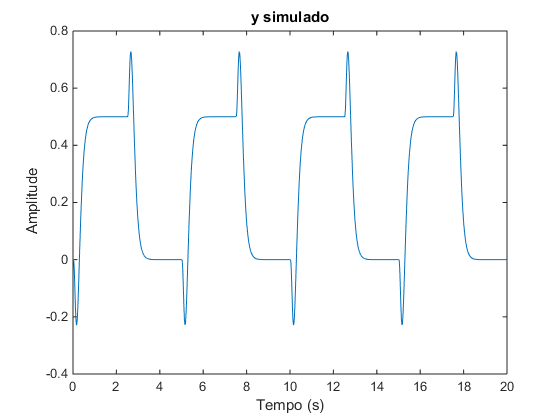
\includegraphics[width=2.5in]{../img/y.png}
\caption{Dados obtidos por Simulink para a variação da saída $(y(t))$ com o tempo}
\label{fig:y_t}
\end{figure}
\begin{figure}[t]
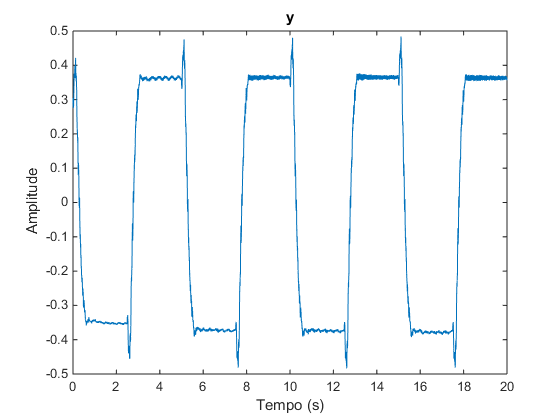
\includegraphics[width=2.5in]{../img/y_dados_01.png}
\caption{Dados obtidos para a saída ($y(t)=\theta(t)+\alpha(t)$) com o sistema real.}
\label{fig:y_d}
\end{figure}
\begin{figure}[t]
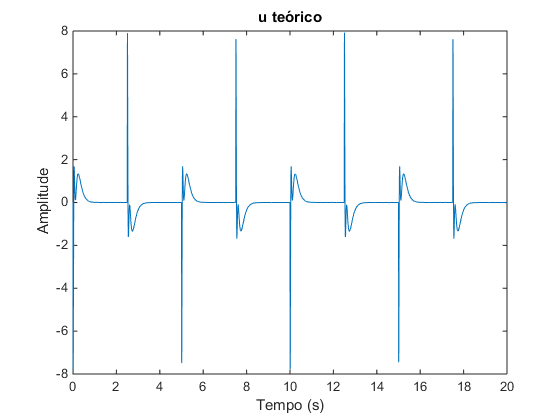
\includegraphics[width=2.5in]{../img/u.png}
\caption{Dados obtidos por Simulink para a variação da saída $(u(t))$ com o tempo}
\label{fig:u_t}
\end{figure}
\begin{figure}[t]
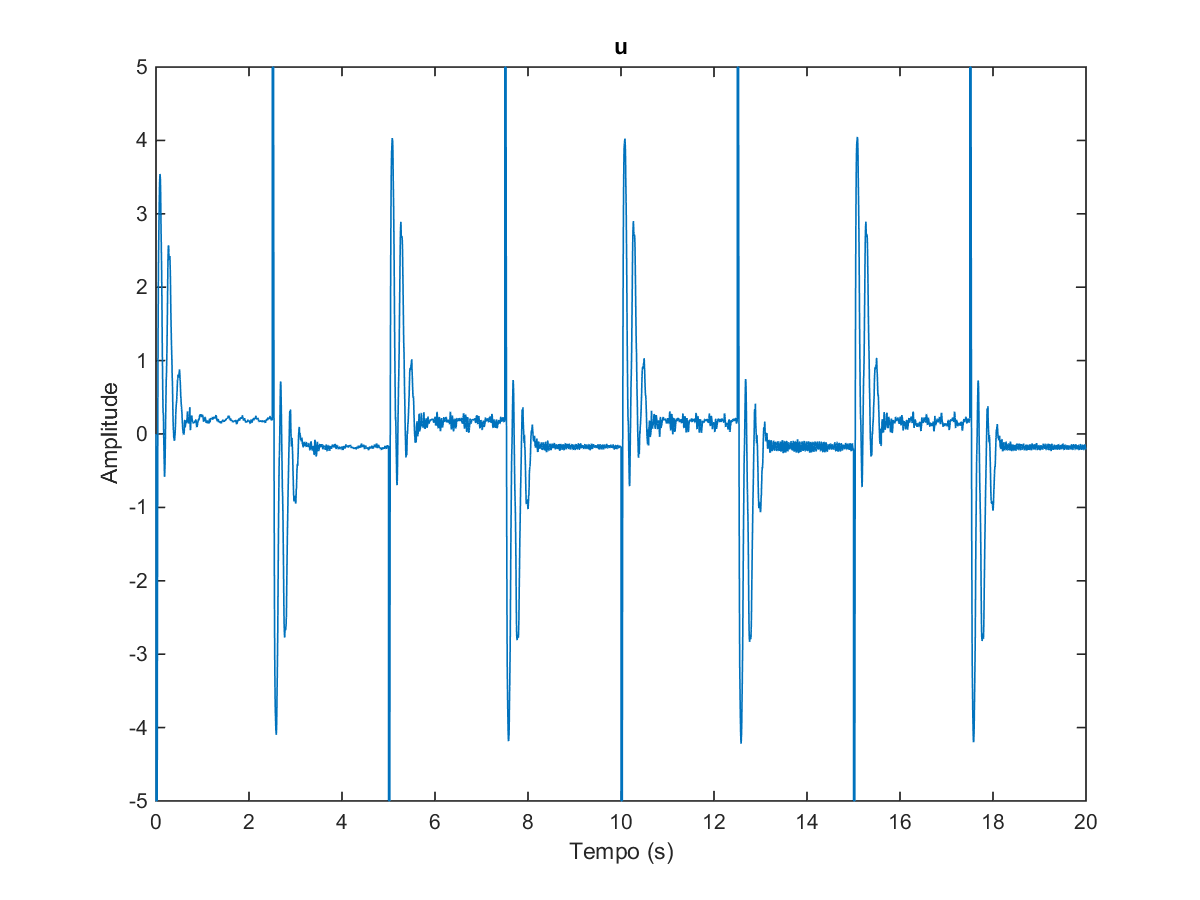
\includegraphics[width=2.5in]{../img/u_dados_01.png}
\caption{Dados obtidos para $u(t)$ com o sistema real}
\label{fig:u_d}
\end{figure}
Quanto à saída obtida observas-se que, apesar de ser muito semelhante à saída obtida através da simulação computacional, na simulação o valor de y tende para valores bem determinados de amplitude sempre que se varia a referência (neste caso, a referência é uma onda quadrada com um período de $T=5$s), enquanto que no sistema real é possivel notar a existência de uma pequena oscilação em torno dos valores onde a barra se deveria encontrar estática. Tal siginfica que quando a barra deveria estar parada, a sua ponta ainda vibra, mesmo que pouco. Tal pode dever-se à zona morta do motor utilizado, visto que o controlador já não consegue fornecer energia suficiente para que o motor actue na barra de modo a esta ficar perfeitamente imóvel.\\
Também comparando os resultados obtidos para u, é possível confirmar a perturbação da zona morta do motor visto que o valor de u, que é o sinal que actua sobre o motor,  na simulação tende para 0 suavemente, enquanto que na prática u varia impulsivamente, o que é uma tentativa do controlador de conseguir controlar o motor fora da sua zona morta. Quando o valor obtido para a ponta da barra finalmente se aproxima à com o valor na referência, o controlador continua a enviar um sinal ao motor para que este actue de modo a anular as vibrações na barra, no entanto como este não responde, o controlador continua a enviar um  sinal u diferente de 0 para actuar o motor, como se vê na figura \ref{fig:u_d}, enquanto que para um motor perfeito, como é o caso da figura \ref{fig:u_t}, o sinal u vai tender assimptóticamente para 0.

\section{Resposta sem filtro na saída}
Anulando o filtro no sinal do extensómetro através do esquema de Simulink, obtive-se o sinal $u$ e $y$ representados nas figuras \ref{fig:u_00} e \ref{fig:y_00} respectivamente.\\
\begin{figure}[t]
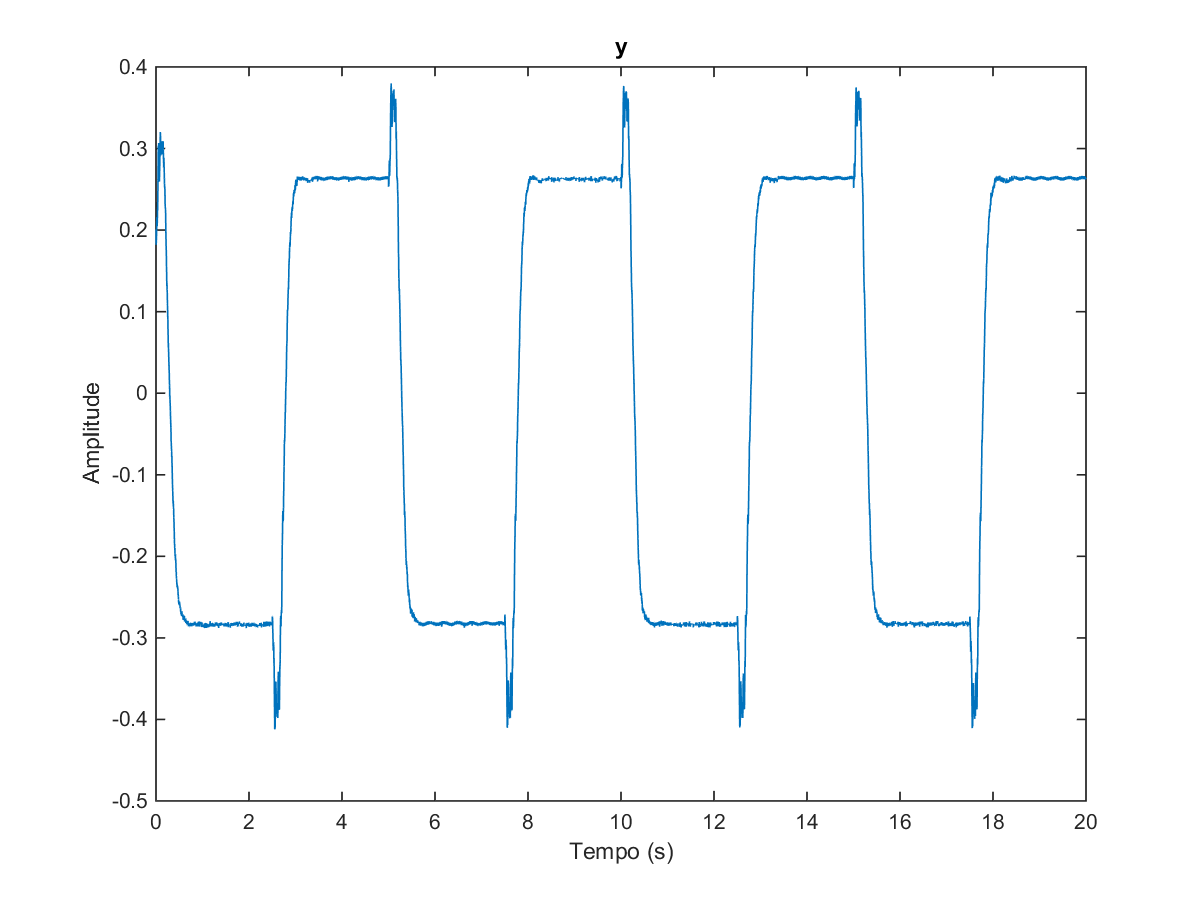
\includegraphics[width=2.5in]{../imgs/dados_00/dados_00_y.png}
\caption{Dados obtidos para $(y)$ sem o filtro no extensómetro}
\label{fig:y_00}
\end{figure}
\begin{figure}[t]
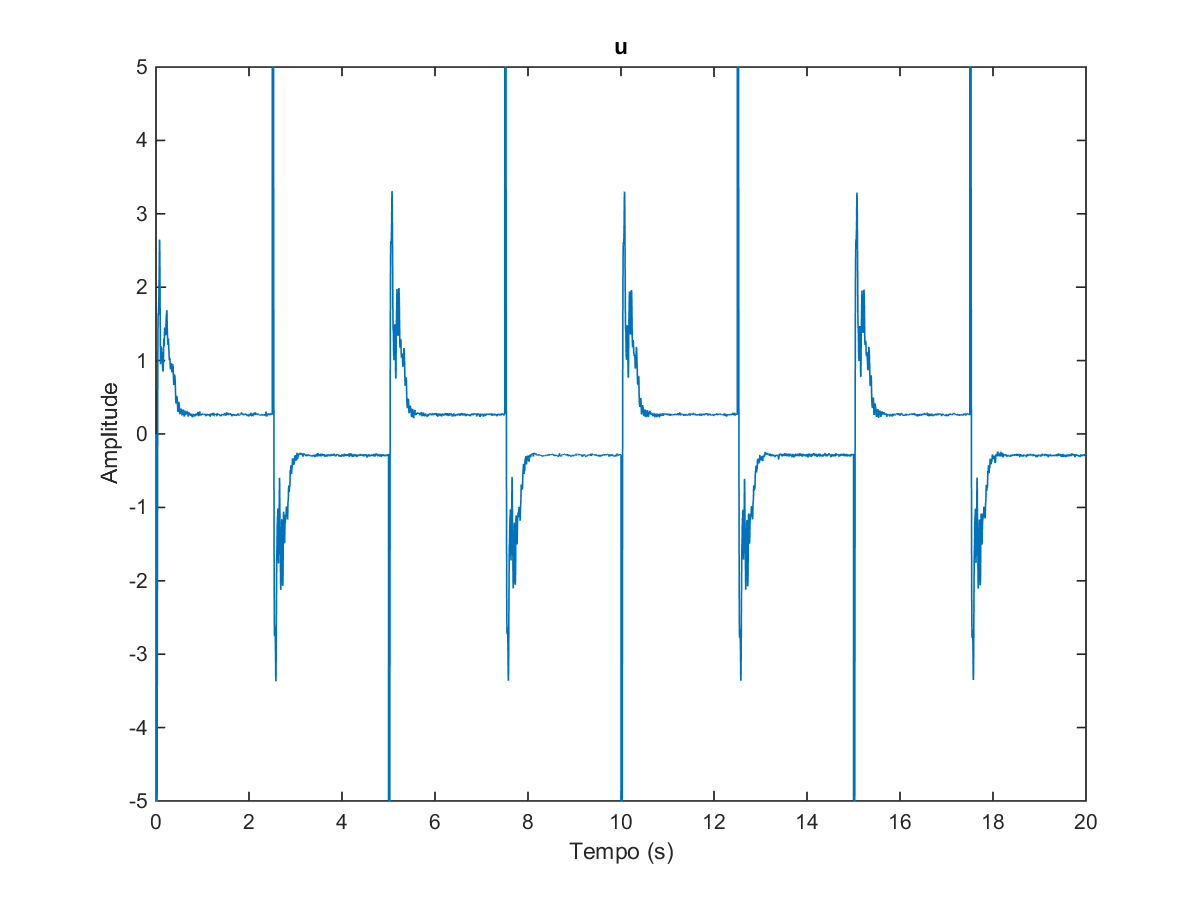
\includegraphics[width=2.5in]{../imgs/dados_00/dados_00_u.png}
\caption{Dados obtidos para $(u)$ com o sistema real}
\label{fig:u_00}
\end{figure}
Nota-se imediatamente que os sinais obtidos são agora mais parecidos com as simulações feitas no Simulink, visto que a introdução de um filtro que elimina as altas frequências num sensor é semelhante a baixar a frequência de amostragem do sensor, pois as variações rápidas que são medidas não chegam ao controlador. Assim sendo, visto que sem filtro a estimação é mais rápida que com o filtro, obtém-se um resultado mais aproximado da simulação (que é ideal).\\
É de notar que , de modo semelhante ao que pode ser observado nos resultados da secção anterior, o sinal $u$ nunca chega a ir exactamente para 0 como é observado na simulação, visto que chega a um ponto que o sinal enviado para corrigir a posição do motor não é suficiente para que este actue, o que resulta num erro na entrada do controlador e consequentemente num sinal $u$ à saída deste diferente de 0.

\section{Efeito da variação do polo do pré-filtro}
A introdução de um filtro passa-baixo na referência irá eliminar as componentes de alta frequência deste sinal, que neste caso, se escolheu ser uma onda quadrada com frequência $f=0.2$Hz. Visto que a onda quadrada varia muito rapidamente, passando quase instantâneamente do seu valor máximo para o seu valor mínimo a cada meio período, isto leva a um comportamento muito impulsivo do sistema (e consequentemente da estrutura de controlo). A filtragem da referência leva a uma suavização deste sinal, resultanto num comportamento mais suave do sistema.\\
Como é possivel observar nas figuras \ref{fig:pf_y}, \ref{fig:pf_u}, \ref{fig:pf_ref}, à medida que se diminui o valor da variável wnpf, vai-se deslocando o pólo deste filtro cada vez mais para a esquerda, sendo que quando wnpf=0, o filtro filtra todas as frequências (sendo a referência 0 para qualquer t). Esta filtragem irá eliminar as altas frequências do sinal de entrada, que estimulam um comportamento muito rápido do sistema, o que implica que quanto menor for a frequência de corte, maior será a suavidade com que o sistema vai tender para a estabilidade.
\begin{figure}[t]
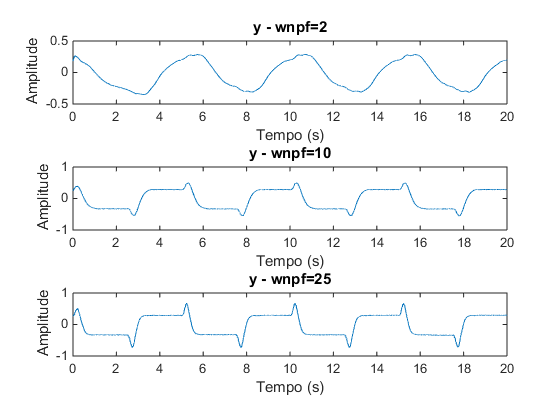
\includegraphics[width=3.5in]{../img/y_filtro.png}
\caption{Dados obtidos para a saída ($y$) do sistema real com vários valores da variável wpfn.}
\label{fig:pf_y}
\end{figure}
\begin{figure}[t]
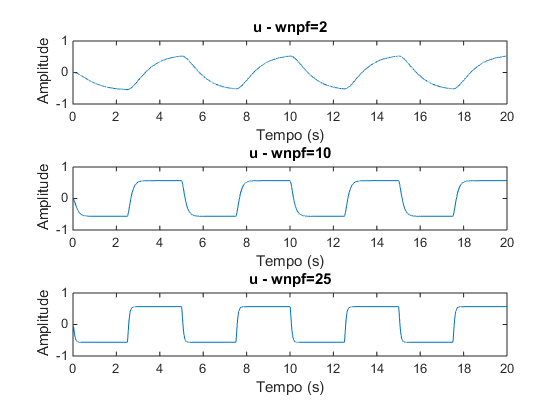
\includegraphics[width=3.5in]{../img/u_filtro.png}
\caption{Dados obtidos para o sinal de actuação ($u$) do sistema real com vários valores da variável wpfn.}
\label{fig:pf_u}
\end{figure}
\begin{figure}[t]
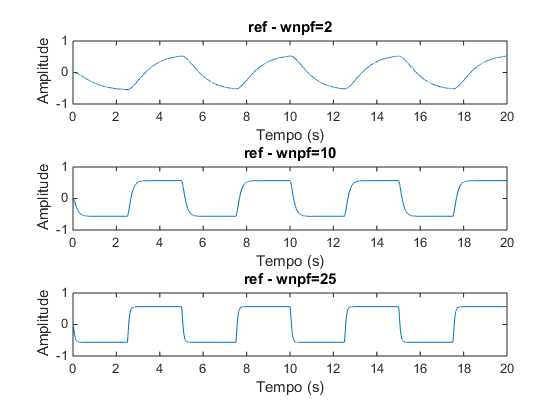
\includegraphics[width=3.5in]{../img/ref_filtro.png}
\caption{Dados obtidos para de referência ($r$) do sistema real com vários valores da variável wpfn}
\label{fig:pf_ref}
\end{figure}
É de realçar que quando o sistema funciona neste regime está-se a atrasar a resposta do sistema face a uma variação externa em troca da sua estabilidade e suavidade. Logo, caso se queira determinar os limites do controlador implementado, não é favorável a implementação de um pré-filtro, da mesma maneira que caso o sistema fosse implementado num sistema comercial, já seria favorável a implementação deste filtro, de modo a conservar os equipamentos controlados.

\section{Ensaio sem sinal do extensómetro}
Os resultados obtidos para a saída do sistema e para a saída do controlador quando o sinal do extensómetro não é utilizado na realimentação apresentam-se nas figuras \ref{fig:y_next} e \ref{fig:u_next}.\\
O sinal na saída do sistema é semelhante ao que foi obtido para o caso em que se implementou um filtro no extensómetro, visto que a eliminação do sinal do extensómetro na realimentação deverá ser equivalente ao caso limite em que o filtro deste corta todas as frequências.\\
Em termos práticos, eliminação do sinal do extensómetro na realimentação significa que o sistema irá perder sensibilidade às variações do ângulo $\alpha$, visto que toda a informação que pode ser obtida acerca deste é a partir da actuação do potenciómetro devido à inércia da barra.

\begin{figure}[t]
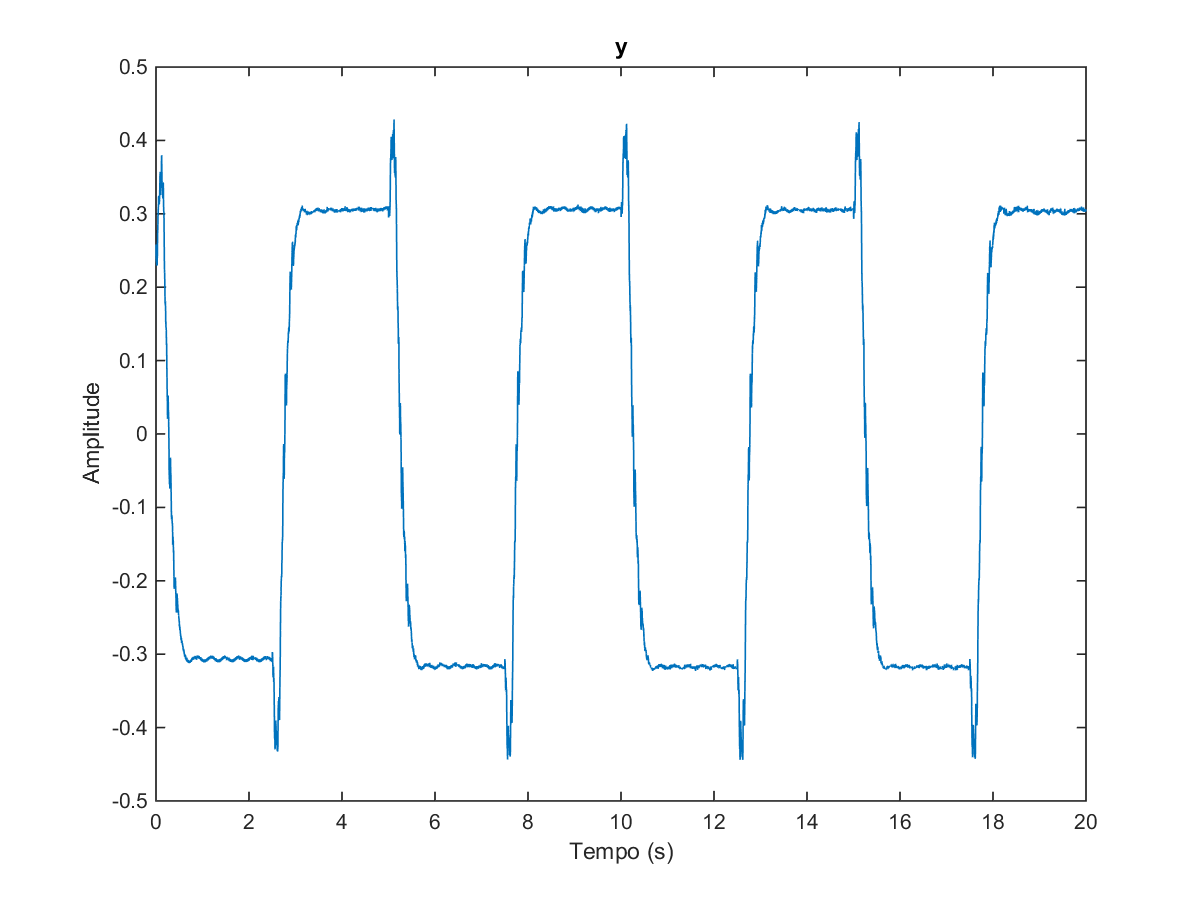
\includegraphics[width=2.5in]{../imgs/dados_0n/dados_0n_y.png}
\caption{Dados obtidos para a saída ($y$) do sistema sem realimentação do extensómetro}
\label{fig:y_next}
\end{figure}
\begin{figure}[t]
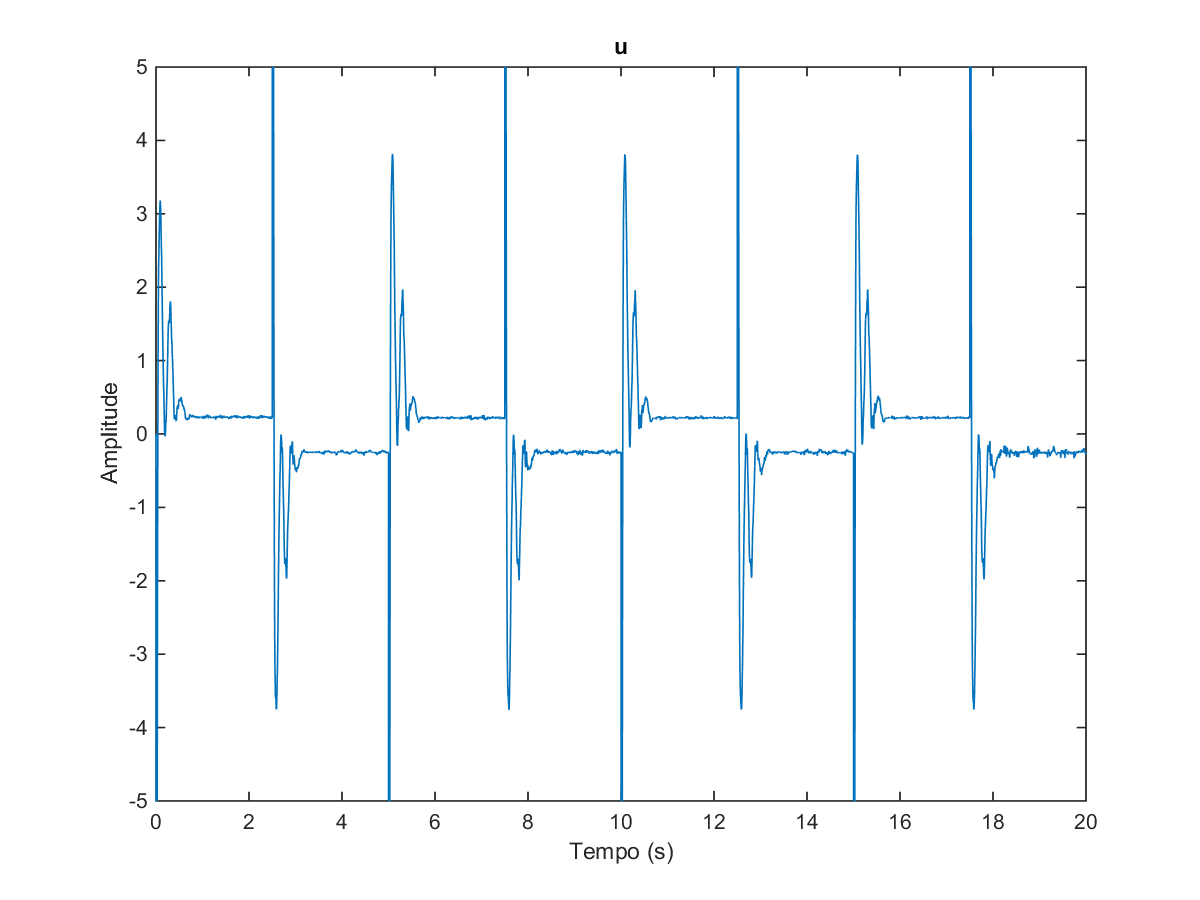
\includegraphics[width=2.5in]{../imgs/dados_0n/dados_0n_u.png}
\caption{Dados obtidos para o sinal de actuação ($u$) do sistema sem realimentação do extensómetro}
\label{fig:u_next}
\end{figure}

\section{Ensaios com outras especificações para os pólos do observador e/ou controlador}
Ensaiou-se o sistema com outros vectores de ganho do controlador e do estimador de modo a obter comportamentos diferentes dos que foram ensaiados anteriormente.\\
\subsection{Primeiro Ensaio}
Utilizou-se para os pólos do controlador:
\begin{equation}
\begin{bmatrix}
-70 & -70  & -10 &-10
\end{bmatrix}
\end{equation}
E para os pólos do observador:
\begin{equation}
\begin{bmatrix}
-75 & -75  & -45 &-45
\end{bmatrix}
\end{equation}
É expectável que com estes pólos se induza um comportamento mais rápido no observador assimptótico, visto que se está a afastar os seus pólos para frequências mais altas comparativamente com o caso analisado nas outras secções.\\
É possível observar que o sinal que sai do controlador ($u$) varia de forma mais impulsiva que com os valores prórpios escolhidos anteriormente. Isto é uma consequência do afastamento dos pólos do observador, que o tornam mais rápido e que por isso induz mais volatilidade na saída do controlador.\\
Na saída do sistema ($y$) não existem diferenças relevantes entre os dois sinais obtidos, pelo que se pode concluir que apesar de se aumentado a rapidez do observador (tornando-o mais sensível às variações de alta frequência), a mecânica do sistema já atingiu o limite para a rapidez de actuação máxima.\\
Os dados obtidos para este ensaio estão representados nas figuras \ref{fig:y_pri} e \ref{fig:u_pri}.
\begin{figure}[t]
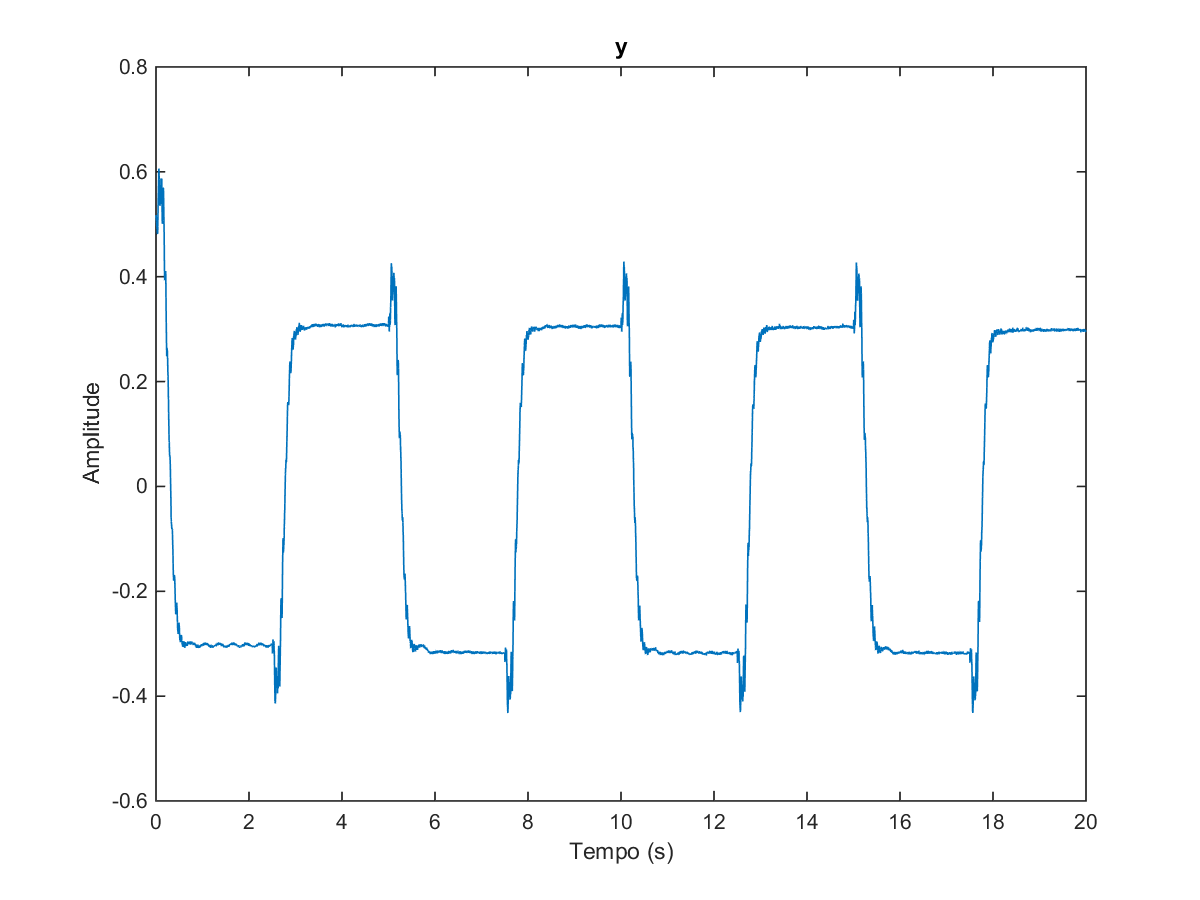
\includegraphics[width=2.5in]{../imgs/dados_00_a/dados_00_a_y.png}
\caption{Dados obtidos para a saída ($y$) do sistema no primeiro ensaio.}
\label{fig:y_pri}
\end{figure}
\begin{figure}[t]
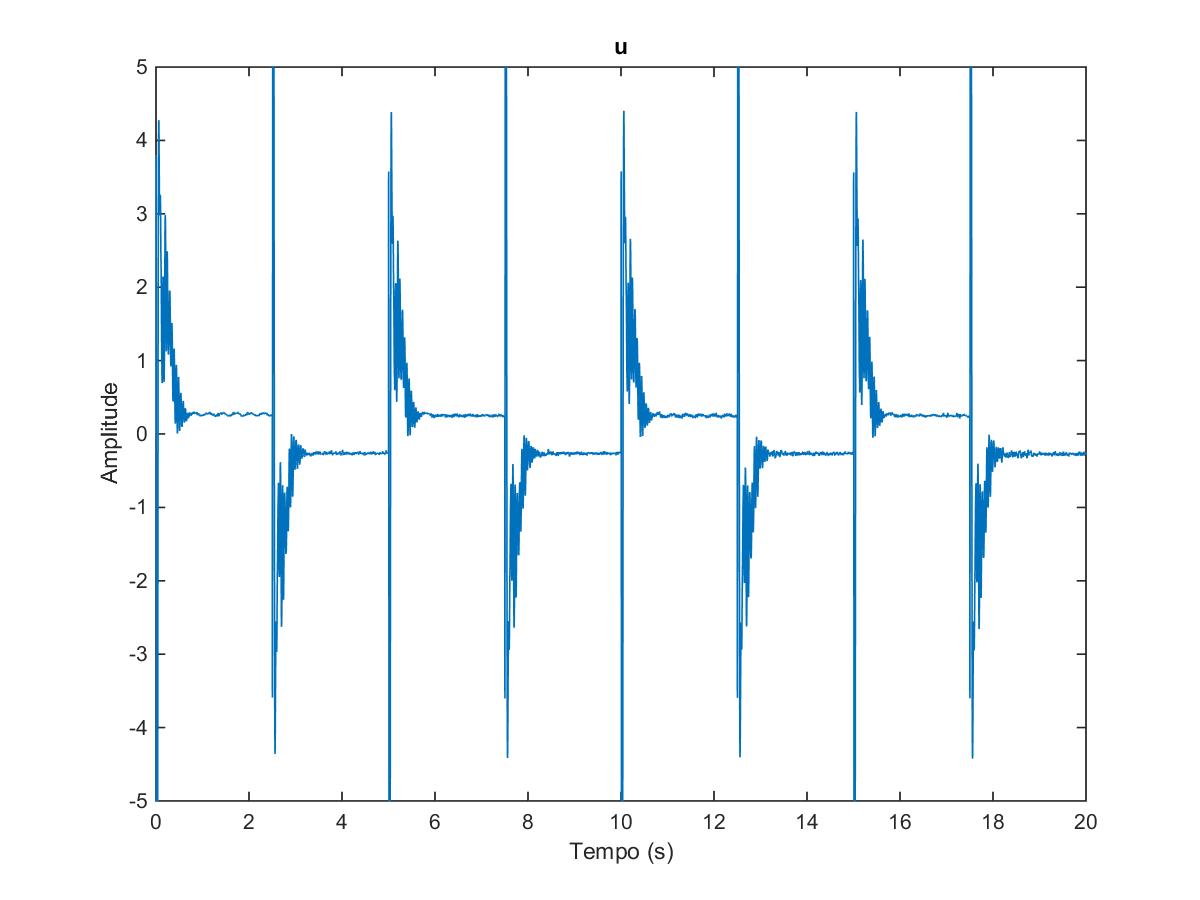
\includegraphics[width=2.5in]{../imgs/dados_00_a/dados_00_a_u.png}
\caption{Dados obtidos para o sinal de actuação ($u$) do sistema no primeiro ensaio}
\label{fig:u_pri}
\end{figure}
\subsection{Segundo Ensaio}
Utilizou-se para os pólos do controlador:
\begin{equation}
\begin{bmatrix}
-70 & -70  & -1+5i &-1+5i
\end{bmatrix}
\end{equation}
E para os pólos do observador:
\begin{equation}
\begin{bmatrix}
-50 & -50  & -30 &-30
\end{bmatrix}
\end{equation}
Espera-se que devido aos pólos complexos do controlador projectado para este ensaio o sinal de actuação varie com uma característica oscilatória amortecida até um certo ponto de estabilidade (onde a saída se anula com a referência).\\
Tal como previsto, o sinal induzido no motor pelo controlador possui uma característica ocilatória amortecida que tende para 0 (quando y tende para a referência).
Quanto ao sinal de saída, devido à actuação do controlador, irá evoluir oscilatóriamente até atingir o valor imposto pela referência, devido novamente à implementação de um controlador com valores próprios complexos.
Os dados obtidos para este ensaio estão representados nas figuras \ref{fig:y_seg} e \ref{fig:u_seg}.
\begin{figure}[t]
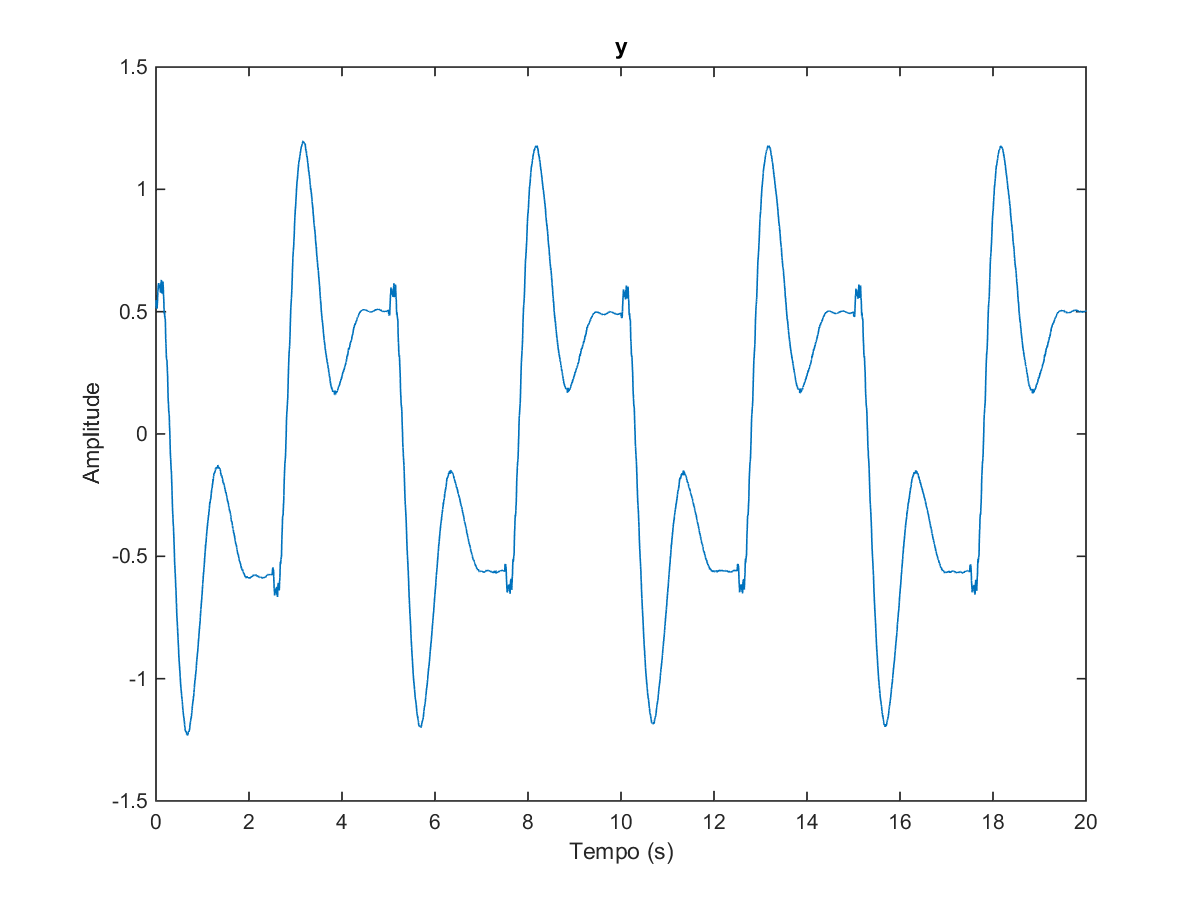
\includegraphics[width=2.5in]{../imgs/dados_00_c/dados_00_c_y.png}
\caption{Dados obtidos para a saída ($y$) do sistema no segundo ensaio.}
\label{fig:y_seg}
\end{figure}
\begin{figure}[t]
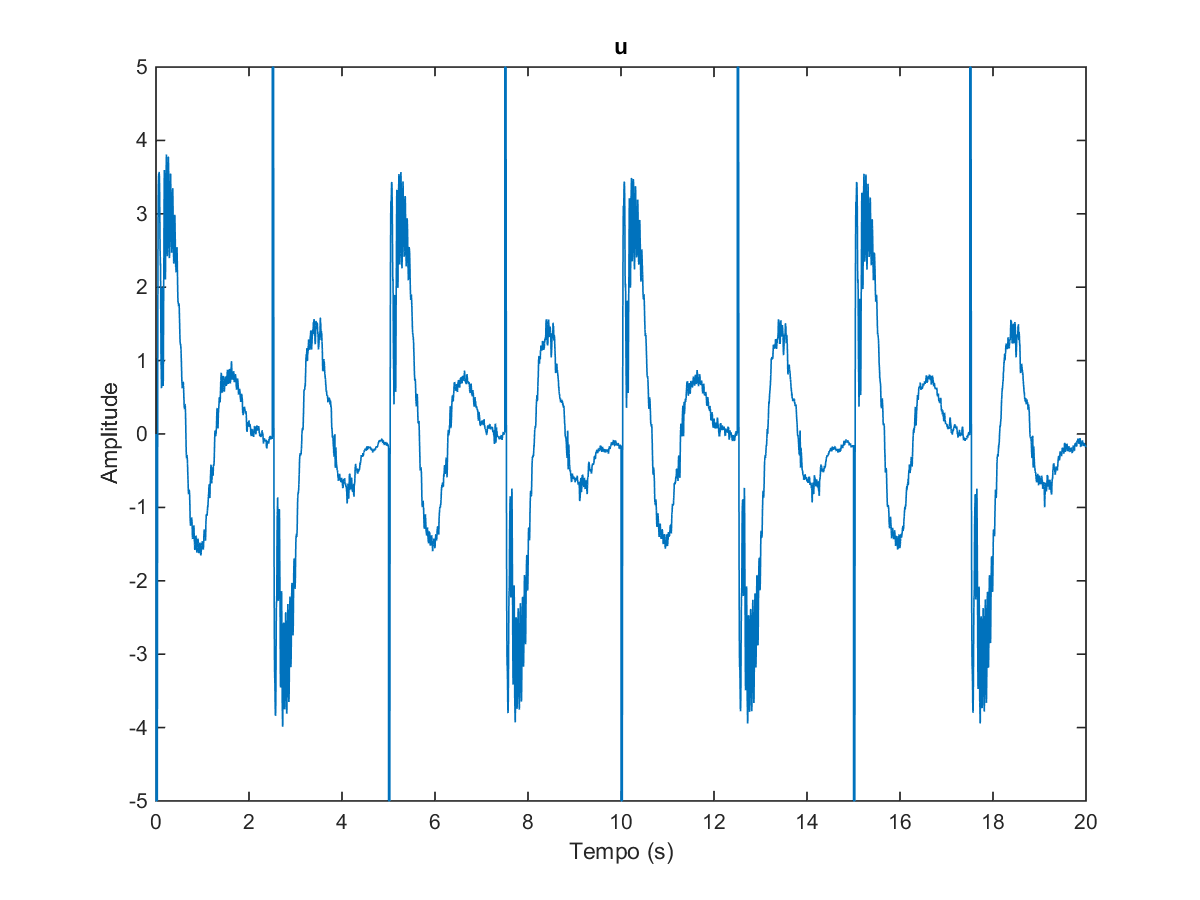
\includegraphics[width=2.5in]{../imgs/dados_00_c/dados_00_c_u.png}
\caption{Dados obtidos para o sinal de actuação ($u$) do sistema no primeiro ensaio}
\label{fig:u_seg}
\end{figure}
\subsection{Terceiro ensaio}
Utilizou-se para os pólos do controlador:
\begin{equation}
\begin{bmatrix}
-20+80i & -20-80i  & -1+5i &-1+5i
\end{bmatrix}
\end{equation}
E para os pólos do observador:
\begin{equation}
\begin{bmatrix}
-50 & -50  & -30 &-30
\end{bmatrix}
\end{equation}
Visto que agora todos os pólos escolhidos para o controlador são complexos, espera-se que o sistema evolua para a estabildade com uma caracterísitica oscilatória amortecida, mas  ao contrário do caso anterior em que apenas metade dos valores próprios do controlador eram complexos, espera-se que haja uma presença mais acentuada do regime oscilatório.\\
Tal pode ser verificado no gráfico da figura \ref{fig:y_e}, em que se observa claramente que a saída do sistema tende para uma oscilação em torno do valor que anula a referência.\\
Este comportamento também pode ser observado na figura \ref{fig:u_e}, onde claramente a amplitude do sinal u, ao contrário dos casos onde não se tem pólos complexos em que u tende exponencialmente para a estabilidade, neste caso u tende para a estabilidade através de um comportamento oscilatório exxponencialmente amortecido, justifica o comportamento do sinal de saída.
\begin{figure}[t]
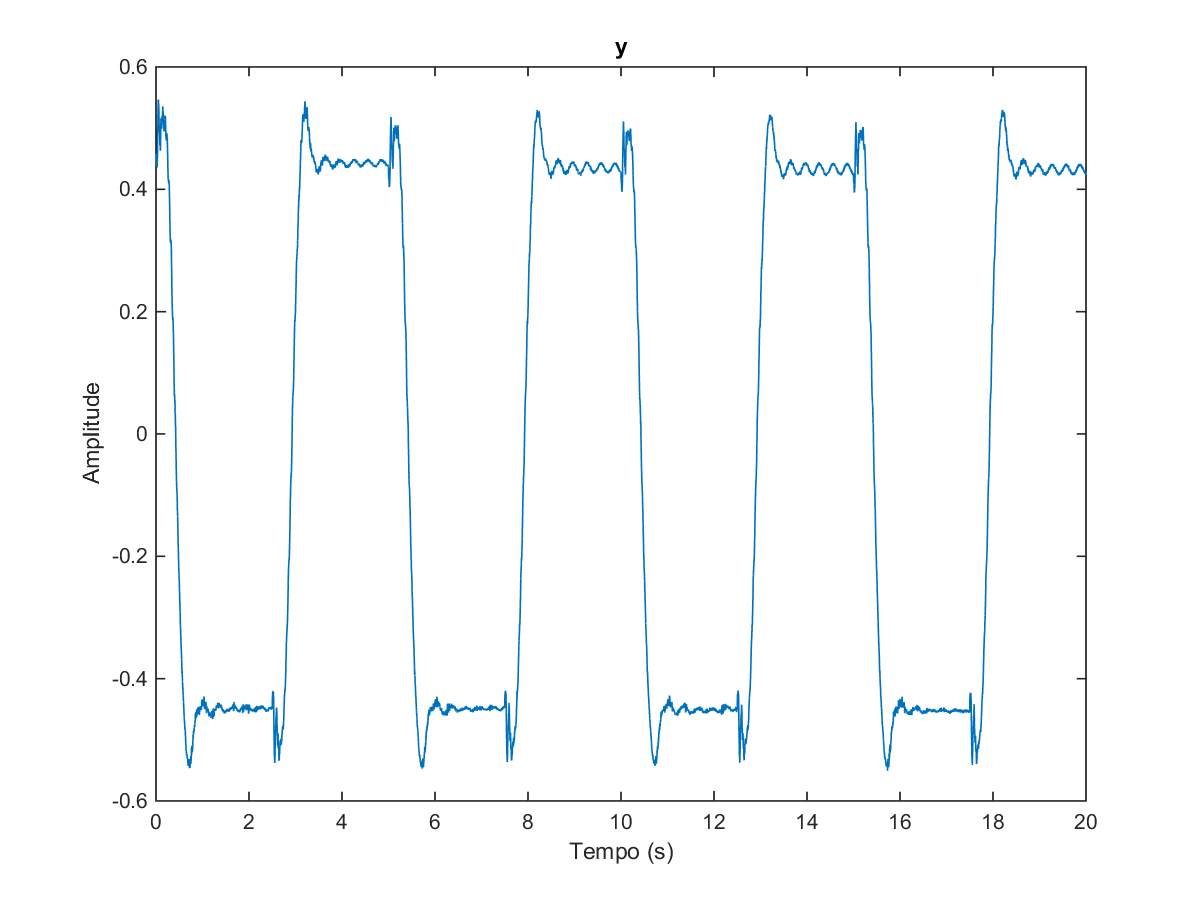
\includegraphics[width=2.5in]{../imgs/dados_00_e/dados_00_e_y.png}
\caption{Dados obtidos para a saída ($y$) do sistema no terceiro ensaio.}
\label{fig:y_e}
\end{figure}
\begin{figure}[t]
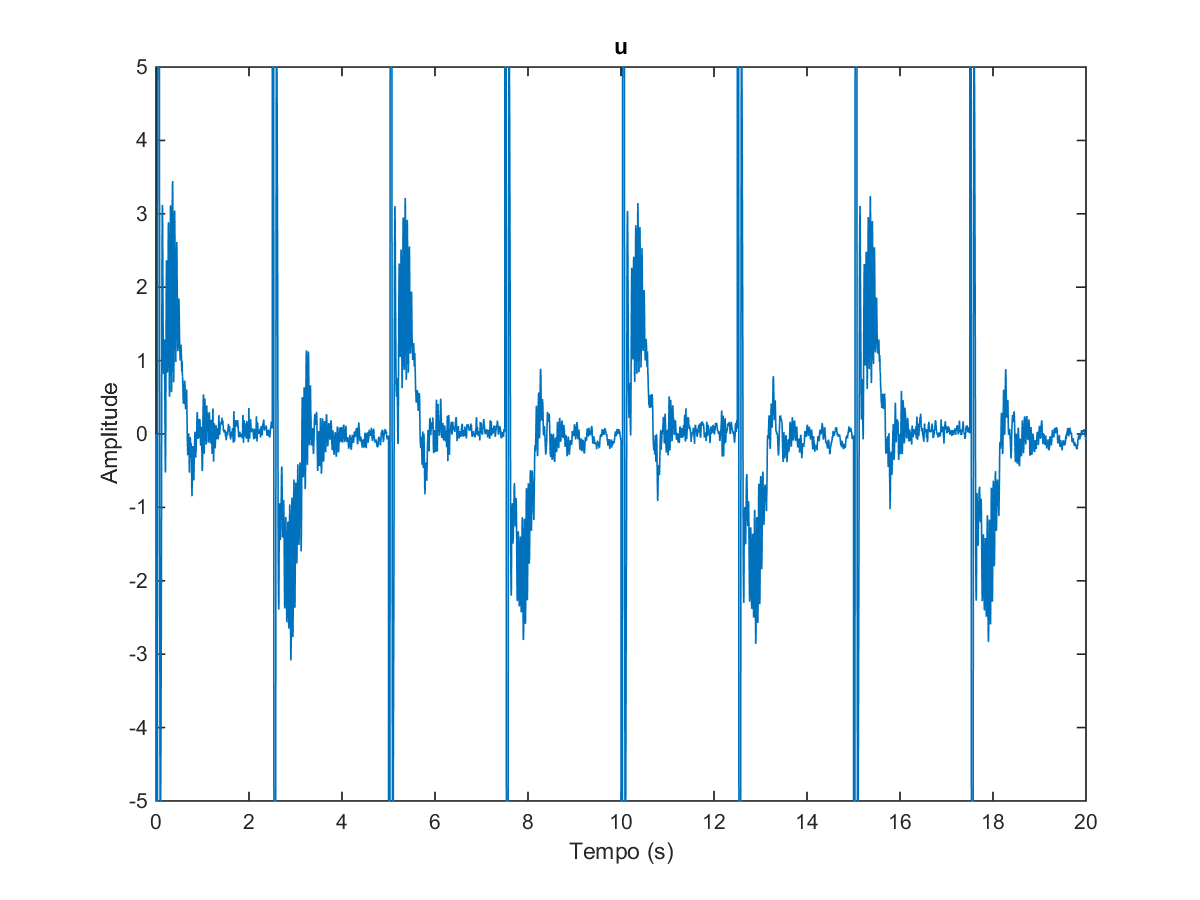
\includegraphics[width=2.5in]{../imgs/dados_00_e/dados_00_e_u.png}
\caption{Dados obtidos para o sinal de actuação ($u$) do sistema no terceiro ensaio}
\label{fig:u_e}
\end{figure}
\subsection{Quarto ensaio}
Utilizou-se para os pólos de controlador:
\begin{equation}
\begin{bmatrix}
-70 & -20 & -10 &-10
\end{bmatrix}
\end{equation}
E para os pólos do observador:
\begin{equation}
\begin{bmatrix}
-50 & -50 & -30+40i &-30-40i
\end{bmatrix}
\end{equation}
Realizou-se este ensaio para tentar perceber qual seria o efeito de aplicar pólos complexos ao observador. Através de uma simulação em Simulink, esperava-se que não existem diferenças relevantes entre este ensaio e o primeiro ensaio.\\
Após realizar o ensaio, cujos gráficos estão representados nas figuras \ref{fig:y_f} e \ref{fig:u_f}, é possivel observar que os resultados obtidos são praticamente iguais aos observados no primeiro ensaio, o que significa que os valores próprios utilizados para o observador no primeiro ensaio são menores em módulo que os que foram utilizados neste ensaio e apenas vieram amplificar a resposta em alta frequência do observador e consequentemente a sua rapidez.
\begin{figure}[t]
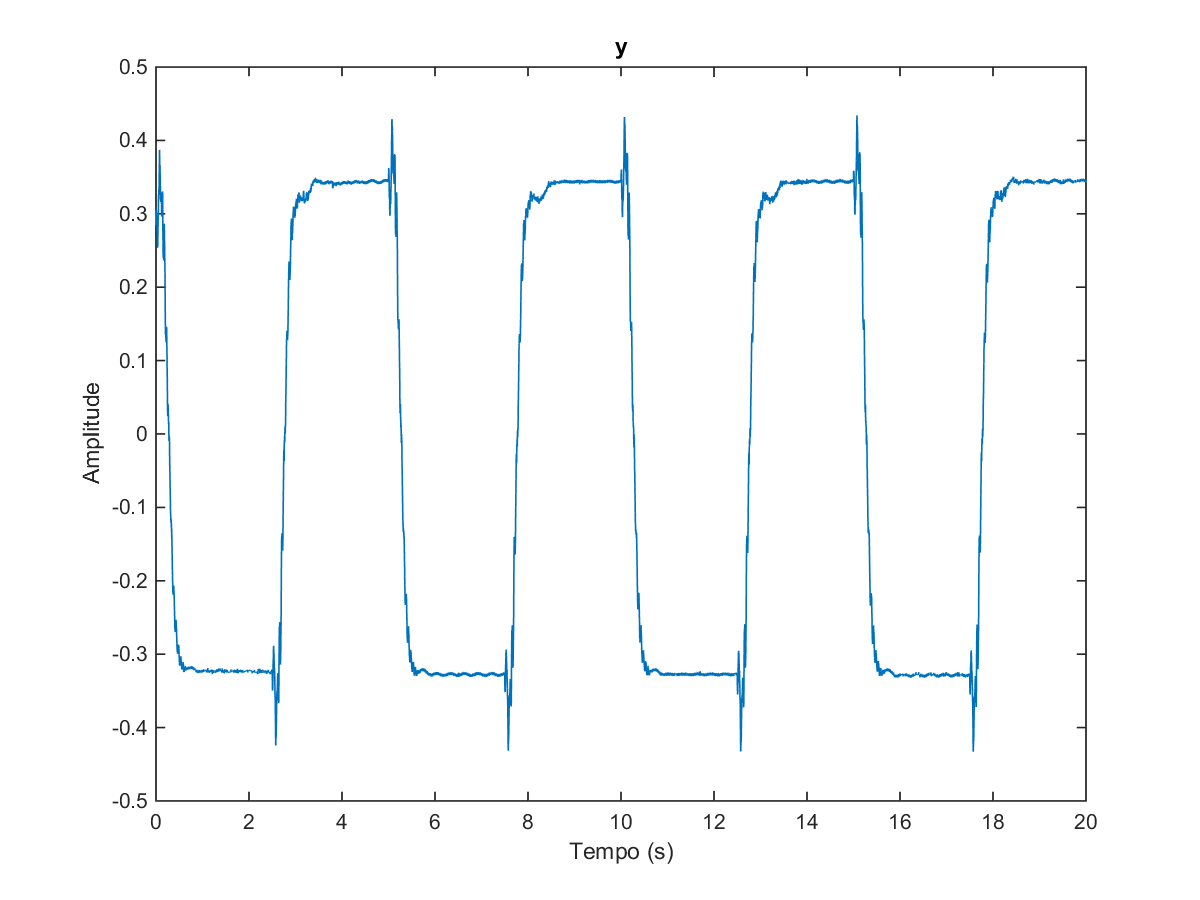
\includegraphics[width=2.5in]{../imgs/dados_00_f/dados_00_f_y.png}
\caption{Dados obtidos para a saída ($y$) do sistema no terceiro ensaio.}
\label{fig:y_f}
\end{figure}
\begin{figure}[t]
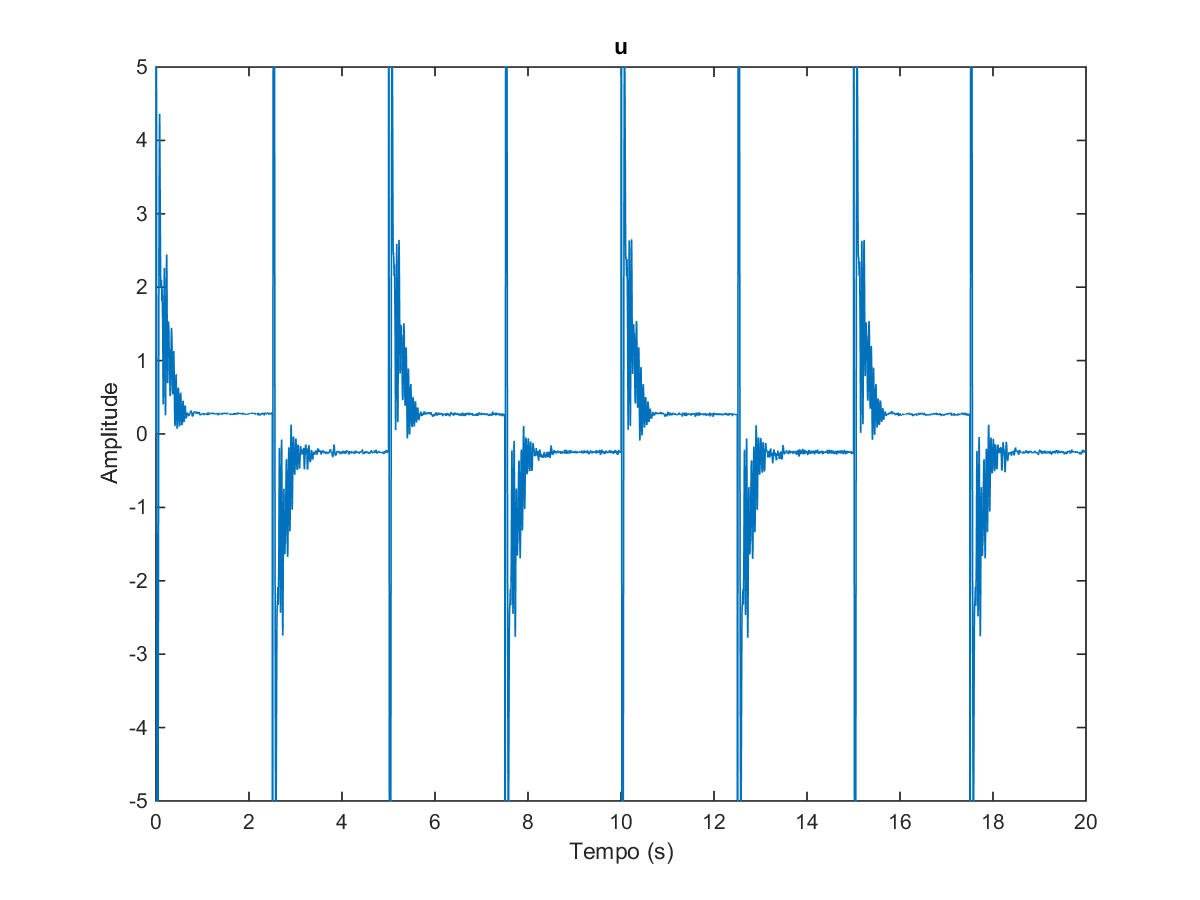
\includegraphics[width=2.5in]{../imgs/dados_00_f/dados_00_f_u.png}
\caption{Dados obtidos para o sinal de actuação ($u$) do sistema no terceiro ensaio}
\label{fig:u_f}
\end{figure}
\subsection{Quinto ensaio}
Foi realizado um último ensaio para apurar qual seria o efeito de colocar todos os pólos, quer do controlador como do observador, como complexos.\\
Utilizou-se para os pólos do controlador:
\begin{equation}
\begin{bmatrix}
-70+40i & -70-40i & -10+10i &-10-10i
\end{bmatrix}
\end{equation}
Utilizou-se para os pólos do observador:
\begin{equation}
\begin{bmatrix}
-50+40i & -50-40i & -30+40i &-30-40i
\end{bmatrix}
\end{equation}
Apesar de os resultados da simulação apontarem para um regime com pouca oscilação, o comportamento obtido foi um regime altamente oscilatório e impulsivo, como pode ser observado nas figuras \ref{fig:y_g} e \ref{fig:u_g}.
Analisando o erro deste ensaio (a entrada do controlador), observa-se que o sistema está a tender no sentido de minimizar o erro (figura \ref{fig:erro}), apesar do seu comportamento altamente oscilatório.
\begin{figure}[t]
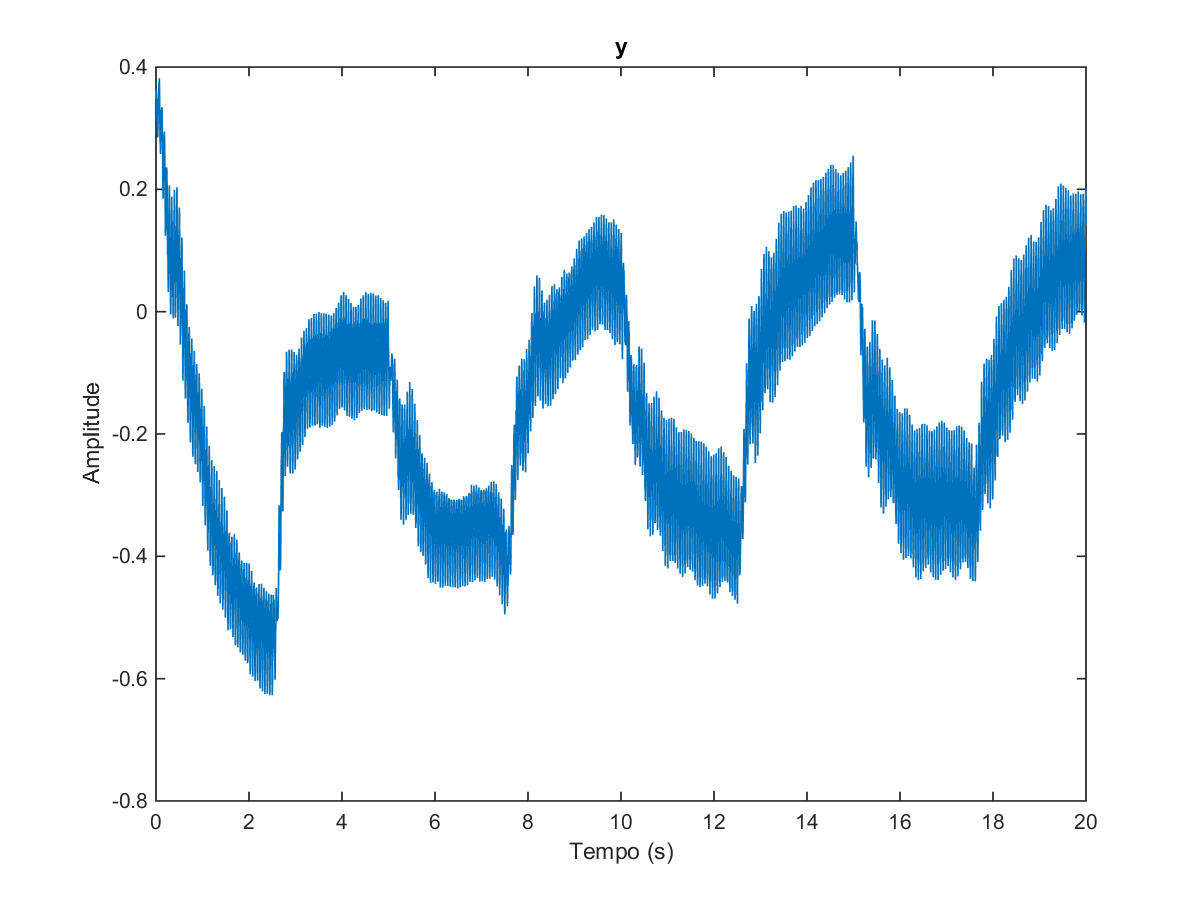
\includegraphics[width=2.5in]{../imgs/dados_00_g/dados_00_g_y.png}
\caption{Dados obtidos para a saída ($y$) do sistema no terceiro ensaio.}
\label{fig:y_g}
\end{figure}
\begin{figure}[t]
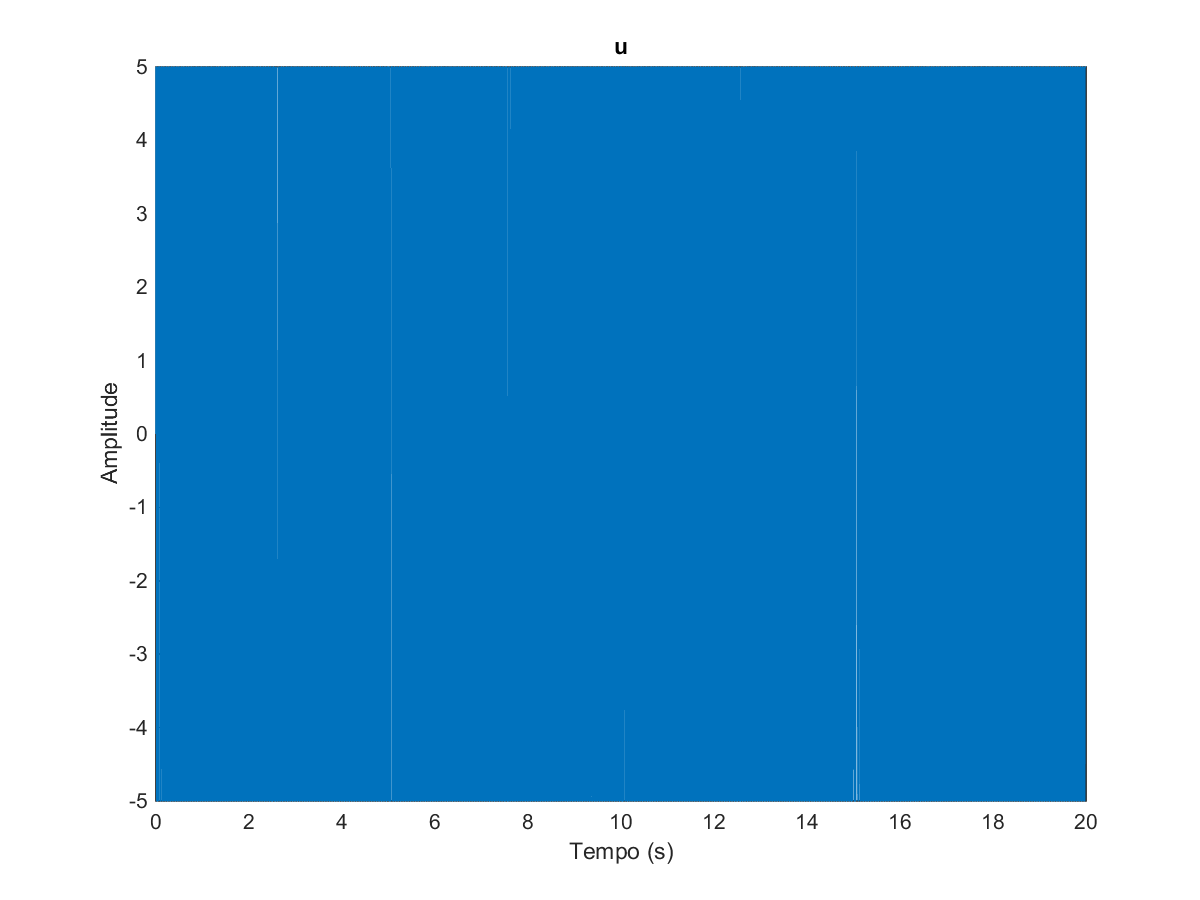
\includegraphics[width=2.5in]{../imgs/dados_00_g/dados_00_g_u.png}
\caption{Dados obtidos para o sinal de actuação ($u$) do sistema no terceiro ensaio}
\label{fig:u_g}
\end{figure}
\begin{figure}[t]
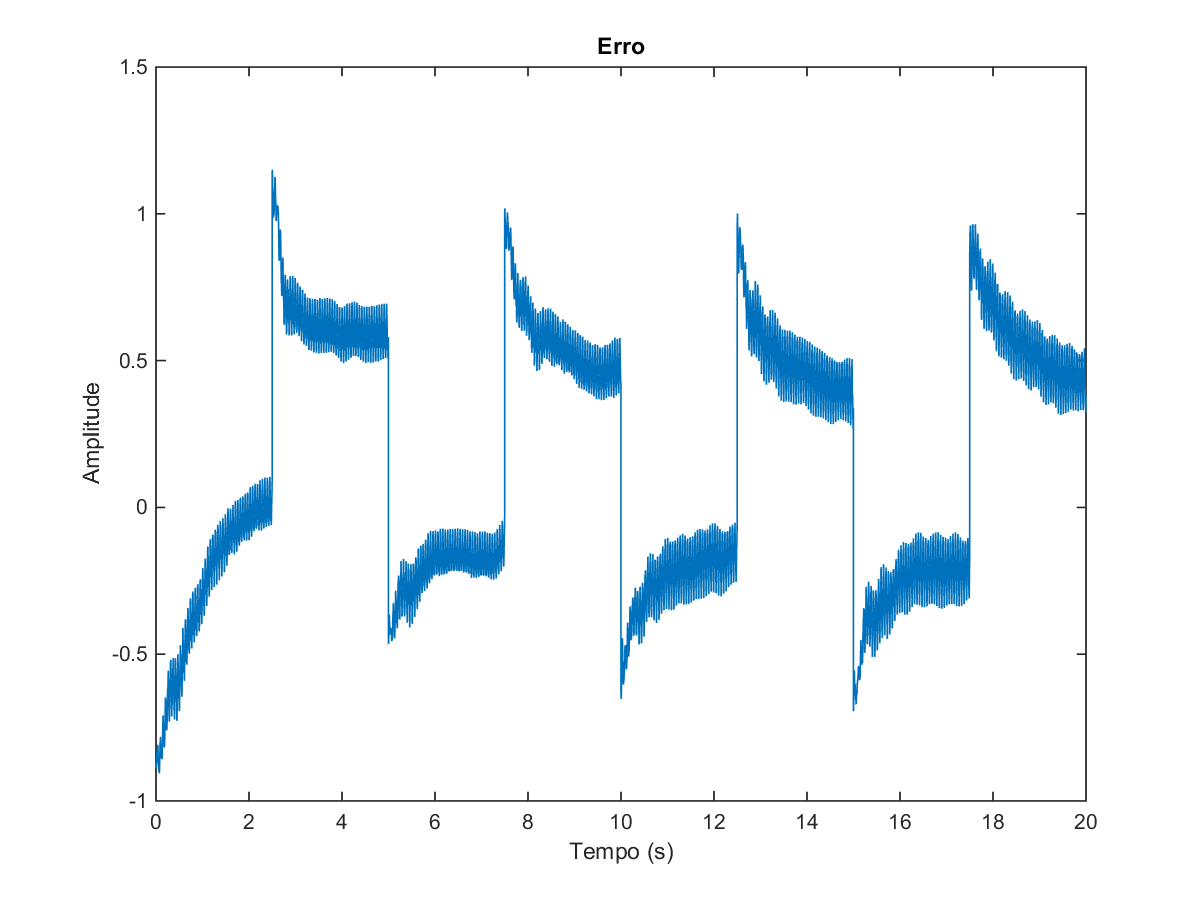
\includegraphics[width=2.5in]{../imgs/dados_00_g/dados_00_g_err.png}
\caption{Dados obtidos para o erro na entada do controlador do sistema no terceiro ensaio}
\label{fig:erro}
\end{figure}
\label{s:conclu}
\section{Conclusões e Críticas}
Como foi referido na comparação do sistema real com o sistema ideal simulado, para a escala de tempo utilizada, o factor que mais contribuiu para o comportamento não ideal do sistema real foi o desvio que se observou no sinal de actuação do sistema (que tende para 0 na simulação mas não tende para 0 quando se ensaio o sistema real). Como foi referido no relatório, tal se deve à zona morta do motor, isto é, a zona em que o sinal de actuação não é suficientemente forte para induzir no motor uma acção mecânica. Isto signfica que o erro (entrada do controlador implementado) irá induzir no controlador uma saída diferente de 0 de modo a actuar o motor para que este se aproxime da referência, no entanto como este sinal de actuação não é suficiente para actuar o motoro erro permanece contante (porque a barra não se move).\\
Propõem-se duas soluções para melhorar o controlador implementado de modo a eliminar este efeito:
\begin{itemize}
\item A utilização de um motor mais sensível
\item A implementação de um efeito integral na entrada do controlador.
\end{itemize}
No primeiro caso, a substituição por um motor mais sensível iria minimizar a zona morta do motor, pelo que seria possivel obter um erro menor visto que se conseguia actuar mecanicamente o motor par avalor mais baixos do sinal de actuação. No entanto isto iria implicar a aquisição um motor mais caro.\\
No segundo caso a implementação do efeito integral implicaria que a entrada do controlador deixaria de ser o erro para passar a ser uma integração do erro o que significa que quando o erro passasse a ser tão pequeno que o controlador não conseguiria induzir um sinal forte o suficiente para actuar o motor, o erro permaneciria constante mas a entrada do controlador aumentaria (ou diminuiria) linearmente com o tempo, o que implica que ao fim de alguns instantes o sinal na entrada do controlador seria o suficiente para que a saída deste actuasse mecanicamente o motor, corrigindo novamente a posição da barra sendo que o sistema iria finalmente estabilizar quando o erro fosse tão pequeno que somente passado um grande intervalo de tempo a entrada do controlador fosse grande o suficiente para que este actuasse o motor.
%Incluir melhorias propostas à experiência
\begin{figure*}[T]
  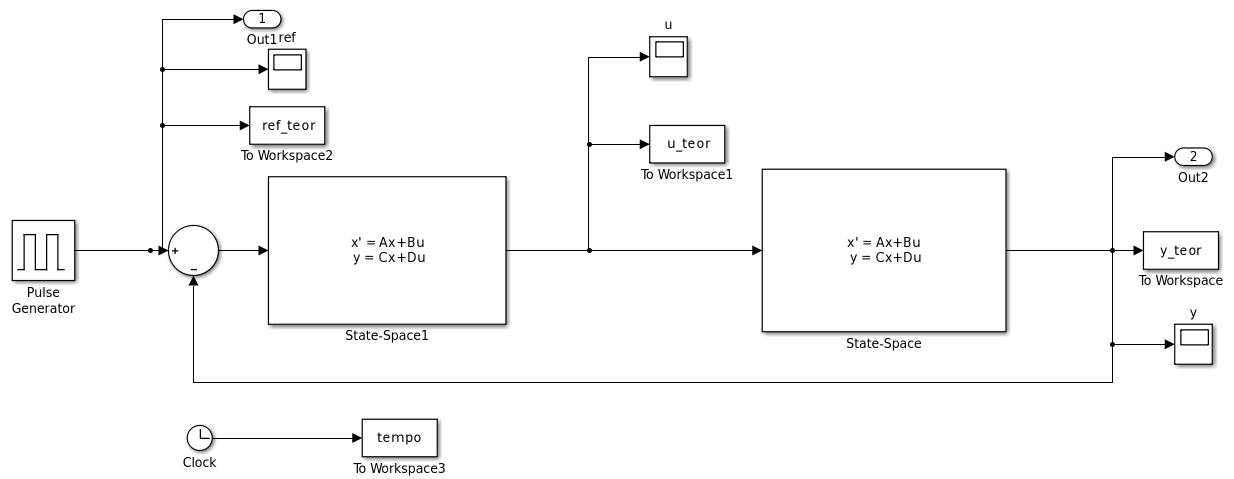
\includegraphics[width=.6\textheight]{../img/simulink.png}% Imports eps image
  \caption{\label{../img/simulink.png} Diagrama da simulação efectuada em {\it simulink}}
\end{figure*}
%\begin{acknowledgments}
%\end{acknowledgments}

%%%%%%%%%%%%%%%%%%%%%%%%%%%%%%%%%%%%%%%%%%%%%%%%%%%%%%%%%%%%%%%%%%%%%%%%%%%%%%%%
% % % % % % % % % % % % % % % %     FIM    % % % % % % % % % % % % % % % % % % % 
%%%%%%%%%%%%%%%%%%%%%%%%%%%%%%%%%%%%%%%%%%%%%%%%%%%%%%%%%%%%%%%%%%%%%%%%%%%%%%%%

\nocite{*}
\bibliography{bibliografia}{}
\bibliographystyle{plain}% Produces the bibliography via BibTeX.
\end{document}
%end of file
